	\documentclass[twoside]{article}
\usepackage{../../estilo-ejercicios}

%--------------------------------------------------------
\begin{document}

\title{Prueba de evaluación continua}
\author{Javier Aguilar Martín}
\maketitle


\begin{ejercicio}{1}
Probar que un grafo simple $G$ es conexo si y solo si el coeficiente de $\lambda$ en su polinomio cromático $P(G;\lambda)$ es no nulo. 
\end{ejercicio}
\begin{solucion}
Supongamos que $G$ no es conexo y se descompone en componentes conexas como $G=G_1\sqcup\cdots \sqcup G_k$. Entonces, $P(G;\lambda)=P(G_1;\lambda)\cdots P(G_k;\lambda)$. Como para cualquier polinomio cromático el término independiente es nulo, en un producto de $k$ polinomios cromáticos, el grado del menor término con coeficiente no nulo es al menos $k$. Como por hipótesis $k\geq 2$, se verifica una de las implicaciones. 

Supongamos ahora que $G$ es conexo. Si $G$ no tiene aristas, entonces $G=K_1$, cuyo polinomio cromático es $P(K_1;\lambda)=\lambda$, y verifica el resultado. Supongamos el resultado cierto para un grafo simple conexo de $m-1$ aristas. Sea entonces $G$ un grafo simple conexo de $m$ aristas. Si $G$ no tiene puentes, entonces es un árbol, cuyo polinomio cromático hemos calculado en los ejercicios y es $\lambda(\lambda-1)^{n-1}$, donde $n$ es el número de vértices, por lo que efectivamente el coeficiente de $\lambda$ no es nulo. Si $G$ no es un árbol, elegimos una arista $e$ que sea un puente, de modo que $P(G;\lambda)=(\lambda-1)P(G/e;\lambda)$. Ahora $G/e$ es un grafo simple (contraer un puente no produce lazos) conexo de $m-1$ aristas, por lo que estamos en la hipótesis de inducción, y al hacer el producto $(\lambda-1)P(G/e;\lambda)$ el coeficiente de $\lambda$ solamente cambia de signo, por lo que sigue sin ser nulo.
\end{solucion}

%\begin{ejercicio}{2}
%Probar que en todo grafo (finito) hay siempre dos vértices con el mismo grado.
%\end{ejercicio}
%\begin{solucion}
%Sea $n=|G|$. El grado de cualquier vértice es a lo sumo $n-1$. Si $G$ es conexo, hay vértices de grado 0, luego los posibles grados son $\{1,\dots, n-1\}$. Como hay $n-1$ grados posibles y $n$ vértices, por el principio del palomar tiene que haber dos vértices del mismo grado. Si $G$ no es conexo, entonces no hay vértices de grado $n-1$, por lo que el conjunto de grados posibles es $\{0,\dots, n-2\}$ y de nuevo es aplicable el principio del palomar.
%\end{solucion}
%
%\begin{ejercicio}{3}
%Sean $H$ y $H'$ dos grafos. El número de Ramsey $R(H,H')$ es el menor $N$ tal que en cualquier 2-coloración (con azul y rojo) de las aristas de $K_N$ existe un subgrafo $H$ azul o un subgrafo $H'$ rojo.
%\begin{enumerate}[a)]
%\item Calcula $R(K_{1,3},K_{1,3})$.
%\item Demuestra que $R(K_{1,3},K_{1,4})>6$. 
%\end{enumerate}
%\end{ejercicio}
%\begin{solucion}\
%\begin{enumerate}[a)]
%\item Para que $K_N$ no contenga un $K_{1,3}$ monocromático no puede haber ningún vértice con 3 aristas del mismo color. Está claro que en $K_6$, al tener cada vértice grado 5, necesariamente llegan siempre al menos 3 aristas del mismo color, por lo que $R(K_{1,3},K_{1,3})\leq 6$. Para ver que se da la igualdad damos la siguiente 2-coloración de aristas de $K_5$:
%
%\definecolor{ffqqqq}{rgb}{1.,0.,0.}
%\definecolor{qqqqff}{rgb}{0.,0.,1.}
%\begin{tikzpicture}[line cap=round,line join=round,>=triangle 45,x=1.0cm,y=1.0cm]
%\clip(-1.28,-0.3333333333333314) rectangle (6.386666666666668,3.42);
%\draw[line width=2.pt,color=qqqqff] (1.,0.) -- (3.,0.) -- (3.618033988749895,1.9021130325903064) -- (2.,3.077683537175253) -- (0.3819660112501053,1.9021130325903073) -- cycle;
%\draw [line width=2.pt,color=qqqqff] (1.,0.)-- (3.,0.);
%\draw [line width=2.pt,color=qqqqff] (3.,0.)-- (3.618033988749895,1.9021130325903064);
%\draw [line width=2.pt,color=qqqqff] (3.618033988749895,1.9021130325903064)-- (2.,3.077683537175253);
%\draw [line width=2.pt,color=qqqqff] (2.,3.077683537175253)-- (0.3819660112501053,1.9021130325903073);
%\draw [line width=2.pt,color=qqqqff] (0.3819660112501053,1.9021130325903073)-- (1.,0.);
%\draw [line width=2.pt,color=ffqqqq] (2.,3.077683537175253)-- (1.,0.);
%\draw [line width=2.pt,color=ffqqqq] (2.,3.077683537175253)-- (3.,0.);
%\draw [line width=2.pt,color=ffqqqq] (0.3819660112501053,1.9021130325903073)-- (3.618033988749895,1.9021130325903064);
%\draw [line width=2.pt,color=ffqqqq] (1.,0.)-- (3.618033988749895,1.9021130325903064);
%\draw [line width=2.pt,color=ffqqqq] (3.,0.)-- (0.3819660112501053,1.9021130325903073);
%\begin{scriptsize}
%\draw [fill=black] (1.,0.) circle (2.5pt);
%\draw [fill=black] (3.,0.) circle (2.5pt);
%\draw [fill=black] (3.618033988749895,1.9021130325903064) circle (2.5pt);
%\draw [fill=black] (2.,3.077683537175253) circle (2.5pt);
%\draw [fill=black] (0.3819660112501053,1.9021130325903073) circle (2.5pt);
%\end{scriptsize}
%\end{tikzpicture}
%
%Como no contiene $K_{1,3}$ monocromático, $R(K_{1,3}, K_{1,3})>5$ y se da la igualdad  $R(K_{1,3}, K_{1,3})=6$. 
%
%\item Basta dar una 2-coloración por aristas de $K_6$ que no contenga $K_{1,3}$ azul ni $K_{1,4}$ rojo:
%
%\definecolor{dcrutc}{rgb}{0.8627450980392157,0.0784313725490196,0.23529411764705882}
%\definecolor{ffqqqq}{rgb}{1.,0.,0.}
%\definecolor{qqqqff}{rgb}{0.,0.,1.}
%\begin{tikzpicture}[line cap=round,line join=round,>=triangle 45,x=1.0cm,y=1.0cm]
%\clip(0.743333333333334,-0.646666666666665) rectangle (10.32666666666668,4.045);
%\draw[line width=2.pt] (4.,0.) -- (6.,0.) -- (7.,1.7320508075688774) -- (6.,3.4641016151377553) -- (4.,3.4641016151377557) -- (3.,1.732050807568879) -- cycle;
%\draw [line width=2.pt,color=qqqqff] (4.,0.)-- (6.,0.);
%\draw [line width=2.pt,color=qqqqff] (6.,0.)-- (7.,1.7320508075688774);
%\draw [line width=2.pt,color=qqqqff] (7.,1.7320508075688774)-- (6.,3.4641016151377553);
%\draw [line width=2.pt,color=qqqqff] (6.,3.4641016151377553)-- (4.,3.4641016151377557);
%\draw [line width=2.pt,color=qqqqff] (4.,3.4641016151377557)-- (3.,1.732050807568879);
%\draw [line width=2.pt,color=qqqqff] (3.,1.732050807568879)-- (4.,0.);
%\draw [line width=2.pt,color=ffqqqq] (3.,1.732050807568879)-- (6.,0.);
%\draw [line width=2.pt,color=ffqqqq] (3.,1.732050807568879)-- (7.,1.7320508075688774);
%\draw [line width=2.pt,color=ffqqqq] (3.,1.732050807568879)-- (6.,3.4641016151377553);
%\draw [line width=2.pt,color=dcrutc] (4.,3.4641016151377557)-- (4.,0.);
%\draw [line width=2.pt,color=ffqqqq] (4.,3.4641016151377557)-- (6.,0.);
%\draw [line width=2.pt,color=ffqqqq] (4.,3.4641016151377557)-- (7.,1.7320508075688774);
%\draw [line width=2.pt,color=ffqqqq] (6.,3.4641016151377553)-- (4.,0.);
%\draw [line width=2.pt,color=ffqqqq] (6.,3.4641016151377553)-- (6.,0.);
%\draw [line width=2.pt,color=ffqqqq] (7.,1.7320508075688774)-- (4.,0.);
%\begin{scriptsize}
%\draw [fill=black] (4.,0.) circle (2.5pt);
%\draw [fill=black] (6.,0.) circle (2.5pt);
%\draw [fill=black] (7.,1.7320508075688774) circle (2.5pt);
%\draw [fill=black] (6.,3.4641016151377553) circle (2.5pt);
%\draw [fill=black] (4.,3.4641016151377557) circle (2.5pt);
%\draw [fill=black] (3.,1.732050807568879) circle (2.5pt);
%\end{scriptsize}
%\end{tikzpicture}
%\end{enumerate}
%\end{solucion}%




%\begin{ejercicio}{1.2}
%Sea $T$ un árbol de orden $p$ que contiene $p_i$ vértices de grado $i$, para cada $i \in\{1,\dots, p-1\}$. Demuestra que $p_1 =
%\sum^{p-1}_{i=3} (i - 2)p_i + 2$.
%\end{ejercicio}
%\begin{solucion}
%%Como $T$ tiene orden $p$, $p_{p-1}\in \{0,1\}$. Si $p_{p-1}=1$ entonces todos los demás vértices son hojas conectadas al vértice de grado $p-1$, es decir, $p_1=p-1$ y $p_i=0$ para $1<i<p-1$. Así, la ecuación resultante sería
%%\[
%%p-1=p-3+2
%%\]
%%que es trivialmente cierta. Supongamos entonces que $p_{p-1}=0$. 
%La ecuación del enunciado se puede reescribir como $\sum_{i=1}^{p-1}(i-2)p_i+2=0$ ya que $p_1$ pasaría a tener coeficiente $-1=1-2$ y $p_2$ tendría coeficiente 0. Ahora la escribimos como
%\[
%\sum_{i=1}^{p-1} i p_i + 2 = \sum_{i=1}^{p-1}2p_i.
%\]
%O lo que es lo mismo
%\[
%\sum_{v\in V(G)}\delta(v)+2=2|V(G)|
%\]
%Por un lado tenemos que al ser un árbol $|V(G)|=|E(G)|+1$ y por otro tenemos que $\sum_{v\in V(G)}\delta(v)=|E(G)|$ por el lema del apretón de manos, de modo que la igualdad es cierta. 
%\end{solucion}
%
%\newpage
%
%\begin{ejercicio}{1.3}
%
%Sea $T$ un árbol de orden $p$ tal que todos sus vértices son de grado 1 o de grado 3. Prueba
%que $T$ contiene exactamente $(p - 2)/2$ vértices de grado 3.
%\end{ejercicio}
%\begin{solucion}
%Basta sustituir en la ecuación del ejercicio anterior, que nos daría $-p_1+p_3+2=0$ junto con la condición $p_1+p_3=p$. 
%\end{solucion}
%
%\newpage
%
%\begin{ejercicio}{1.4}
%
%Encuentra todos los árboles $T$ tales que su complementario $\overline{T}$ es también un árbol.
%\end{ejercicio}
%\begin{solucion}
%Un árbol de $n$ vértices tiene $n-1$ aristas. Además, para un conjunto de $n$ vértices hay $\binom{n}{2}$ posibles aristas. Para que el complementario de un árbol sea también un árbol debería darse $\binom{n}{2}-(n-1)=(n-1)$, lo que nos da $n(n-1)=4(n-1)$. Esto se cumple para $n=1$ y $n=4$, luego tenemos el árbol trivial y los árboles de 4 vértices, que salvo isomorfismo son los dos que aparecen dibujados.
%
%\begin{tikzpicture}[line cap=round,line join=round,>=triangle 45,x=1.0cm,y=1.0cm]
%\clip(-3.2672,3.8856) rectangle (11.4528,5.592);
%\draw [line width=2.pt] (0.,5.)-- (3.,5.);
%\draw [line width=2.pt] (4.,5.)-- (6.,5.);
%\draw [line width=2.pt] (5.,5.)-- (5.,4.);
%\begin{scriptsize}
%\draw [fill=black] (0.,5.) circle (2.5pt);
%\draw [fill=black] (1.,5.) circle (2.5pt);
%\draw [fill=black] (2.,5.) circle (2.5pt);
%\draw [fill=black] (3.,5.) circle (2.5pt);
%\draw [fill=black] (4.,5.) circle (2.5pt);
%\draw [fill=black] (6.,5.) circle (2.5pt);
%\draw [fill=black] (5.,5.) circle (2.5pt);
%\draw [fill=black] (5.,4.) circle (2.5pt);
%\end{scriptsize}
%\end{tikzpicture}
%
%\end{solucion}
%
%\newpage
%
%\begin{ejercicio}{1.5}
%
%Demuestra que todo árbol $T$ tiene un número de hojas mayor o igual que el grado máximo
%de $T$.
%\end{ejercicio}
%\begin{solucion}
%Trivial: considerar el vértice de grado máximo, en el peor de los casos todas las hojas están conectadas a este vértice, en otros casos de los vértices adyacentes saldrán más hojas. 
%\end{solucion}
%
%\newpage
%
%\begin{ejercicio}{1.6}
%Prueba que si $G$ es un grafo conexo de orden $p$ tal que todo subgrafo suyo de tamaño
%$p -1$ es un árbol ``spanning'', entonces $G$ es un árbol o un ciclo.
%\end{ejercicio}
%\begin{solucion}
%Si $G$ no es un árbol ni un ciclo, entonces contiene un grafo formado por un ciclo y una arista  con un vértice de grado 1. A este tipo de grafo lo vamos a llamar $J_n$, con $n$ dependiendo el orden del ciclo. En el caso de que este sea todo el grado, podemos conseguir un subgrafo de tamaño $p-1$ que no es un árbol spanning, esto es, el ciclo que contiene. Si el grafo es mayor, basta aislar partes del grafo que sean $J_n$ hasta que quede como unión de un árbol o un ciclo y grafos $J_n$.
%\end{solucion}
%
%\newpage
%
%\begin{ejercicio}{1.7}
%Prueba o refuta el siguiente enunciado: Si $G$ es un grafo conexo tal que dos cualesquiera
%de sus árboles ``spanning'' son isomorfos, entonces $G$ es un árbol o un ciclo.
%\end{ejercicio}
%\begin{solucion}
%Razonamos de igual manera que en el ejercicio anterior. Es claro que $J_n$ tiene siempre dos árboles spanning no isomorfos, uno en el que tomamos la arista suelta y vamos rodeando el ciclo hasta dejar solo una arista fuera, y otra en la que empezando por la arista suelta añadimos aristas del ciclo a izquierda y derecha hasta que solo falte una por añadir. Cualquier grafo que lo contenga tendrá más de una clase de isomorfismo de árbol maximal, por lo que para que solo tenga un árbol spanning salvo isomorfismo tendrá que ser un árbol o un ciclo. 
%\end{solucion}
%
%\newpage
%
%\begin{ejercicio}{1.8}
%Obtén un árbol spanning por el algoritmo DFS del grafo de Grotzsch de la figura adjunta.
%\end{ejercicio}
%\begin{solucion}
%
%Damos la lista de vértices que se va produciendo y luego añadimos un dibujo del árbol spanning. 
%\[
%[v_1], [v_1,v_2], [v_1,v_2,v_3], [v_1,v_2, v_3, v_4], [v_1,v_2, v_3, v_4, v_5], [v_1,v_2, v_3, v_4, v_6], [v_1,v_2, v_3, v_4, v_6, v_{11}], 
%\]
%\[
%[v_1,v_2, v_3, v_4, v_6, v_{11}, v_7], [v_1,v_2, v_3, v_4, v_6, v_{11}], [v_1,v_2, v_3, v_4, v_6, v_{11}, v_8], [v_1,v_2, v_3, v_4, v_6, v_{11}]
%\]
%\[
%[v_1,v_2, v_3, v_4, v_6, v_{11}], [v_1,v_2, v_3, v_4, v_6, v_{11}, v_9], [v_1,v_2, v_3, v_4, v_6, v_{11}], [v_1,v_2, v_3, v_4, v_6, v_{11}, v_{10}]
%\]
%A partir de entonces la lista se va vaciando sin volver a añadir ningún vértice. El resultado es el siguiente
%
%\definecolor{qqqqff}{rgb}{0.,0.,1.}
%\begin{tikzpicture}[line cap=round,line join=round,>=triangle 45,x=1.0cm,y=1.0cm]
%\clip(-3.742666666666666,-0.7253333333333322) rectangle (8.470666666666665,5.28);
%\draw[line width=2.pt] (0.,0.) -- (3.,0.) -- (3.9270509831248424,2.85316954888546) -- (1.5,4.616525305762879) -- (-0.9270509831248419,2.853169548885461) -- cycle;
%\draw [line width=2.pt] (0.,0.)-- (3.,0.);
%\draw [line width=2.pt] (3.,0.)-- (3.9270509831248424,2.85316954888546);
%\draw [line width=2.pt] (3.9270509831248424,2.85316954888546)-- (1.5,4.616525305762879);
%\draw [line width=2.pt] (1.5,4.616525305762879)-- (-0.9270509831248419,2.853169548885461);
%\draw [line width=2.pt] (-0.9270509831248419,2.853169548885461)-- (0.,0.);
%\draw [line width=2.pt] (-0.9270509831248419,2.853169548885461)-- (3.,0.);
%\draw [line width=2.pt] (-0.9270509831248419,2.853169548885461)-- (3.9270509831248424,2.85316954888546);
%\draw [line width=2.pt] (1.5,4.616525305762879)-- (0.,0.);
%\draw [line width=2.pt] (1.5,4.616525305762879)-- (3.,0.);
%\draw [line width=2.pt] (0.,0.)-- (3.9270509831248424,2.85316954888546);
%\draw [line width=2.pt] (1.5,2.8531695488854605)-- (1.5,2.04);
%\draw [line width=2.pt] (1.5,2.04)-- (0.7498492564294226,2.3077987118759378);
%\draw [line width=2.pt] (1.0129721070609903,1.443660268553074)-- (1.5,2.04);
%\draw [line width=2.pt] (1.5,2.04)-- (2.0449101167030137,1.4857141657331447);
%\draw [line width=2.pt] (1.5,2.04)-- (2.2515228718441938,2.303575735277337);
%\draw (1.313333333333333,5.194666666666663) node[anchor=north west] {$v_1$};
%\draw (4.2253333333333325,3.104) node[anchor=north west] {$v_2$};
%\draw (3.414666666666666,0.096) node[anchor=north west] {$v_3$};
%\draw (-0.45733333333333326,-0.1706666666666659) node[anchor=north west] {$v_4$};
%\draw (-1.396,3.232) node[anchor=north west] {$v_5$};
%\draw (1.505333333333333,2.976) node[anchor=north west] {$v_6$};
%\draw (2.252,2.432) node[anchor=north west] {$v_7$};
%\draw (2.049333333333333,1.6106666666666658) node[anchor=north west] {$v_8$};
%\draw (1.0146666666666664,1.568) node[anchor=north west] {$v_9$};
%\draw (0.,2.432) node[anchor=north west] {$v_{10}$};
%\draw (1.505333333333333,2.165333333333332) node[anchor=north west] {$v_{11}$};
%\draw [line width=2.8pt,color=qqqqff] (1.5,4.616525305762879)-- (3.9270509831248424,2.85316954888546);
%\draw [line width=2.8pt,color=qqqqff] (3.9270509831248424,2.85316954888546)-- (3.,0.);
%\draw [line width=2.8pt,color=qqqqff] (3.,0.)-- (0.,0.);
%\draw [line width=2.8pt,color=qqqqff] (0.,0.)-- (-0.9270509831248419,2.853169548885461);
%\draw [line width=2.8pt,color=qqqqff] (-0.9270509831248419,2.853169548885461)-- (1.5,2.8531695488854605);
%\draw [line width=2.8pt,color=qqqqff] (1.5,2.8531695488854605)-- (1.5,2.04);
%\draw [line width=2.8pt,color=qqqqff] (1.5,2.04)-- (2.2515228718441938,2.303575735277337);
%\draw [line width=2.8pt,color=qqqqff] (1.5,2.04)-- (2.0449101167030137,1.4857141657331447);
%\draw [line width=2.8pt,color=qqqqff] (1.5,2.04)-- (1.0129721070609903,1.443660268553074);
%\draw [line width=2.8pt,color=qqqqff] (1.5,2.04)-- (0.7498492564294226,2.3077987118759378);
%\begin{scriptsize}
%\draw [fill=black] (0.,0.) circle (2.0pt);
%\draw [fill=black] (3.,0.) circle (2.5pt);
%\draw [fill=black] (3.9270509831248424,2.85316954888546) circle (2.0pt);
%\draw [fill=black] (1.5,4.616525305762879) circle (2.0pt);
%\draw [fill=black] (-0.9270509831248419,2.853169548885461) circle (2.0pt);
%\draw [fill=black] (0.7498492564294226,2.3077987118759378) circle (2.5pt);
%\draw [fill=black] (1.5,2.8531695488854605) circle (2.5pt);
%\draw [fill=black] (2.2515228718441938,2.303575735277337) circle (2.5pt);
%\draw [fill=black] (2.0449101167030137,1.4857141657331447) circle (2.5pt);
%\draw [fill=black] (1.0129721070609903,1.443660268553074) circle (2.5pt);
%\draw [fill=black] (1.5,2.04) circle (2.5pt);
%\end{scriptsize}
%\end{tikzpicture}
%
%
%
%\end{solucion}
%\newpage
%
%\begin{ejercicio}{1.9}
%Obtén un árbol spanning por el algoritmo DFS del grafo de Petersen de la figura adjunta.
%\end{ejercicio}
%\begin{solucion}\
%
%\definecolor{qqqqff}{rgb}{0.,0.,1.}
%\begin{tikzpicture}[line cap=round,line join=round,>=triangle 45,x=1.0cm,y=1.0cm]
%\clip(-3.796,-0.928) rectangle (8.417333333333332,5.077333333333329);
%\draw[line width=2.pt] (0.,0.) -- (3.,0.) -- (3.9270509831248424,2.85316954888546) -- (1.5,4.616525305762879) -- (-0.9270509831248419,2.853169548885461) -- cycle;
%\draw [line width=2.pt] (0.,0.)-- (3.,0.);
%\draw [line width=2.pt] (3.,0.)-- (3.9270509831248424,2.85316954888546);
%\draw [line width=2.pt] (3.9270509831248424,2.85316954888546)-- (1.5,4.616525305762879);
%\draw [line width=2.pt] (1.5,4.616525305762879)-- (-0.9270509831248419,2.853169548885461);
%\draw [line width=2.pt] (-0.9270509831248419,2.853169548885461)-- (0.,0.);
%\draw (1.313333333333333,5.194666666666663) node[anchor=north west] {$v_1$};
%\draw (4.2253333333333325,3.104) node[anchor=north west] {$v_2$};
%\draw (3.414666666666666,0.096) node[anchor=north west] {$v_3$};
%\draw (-0.45733333333333326,-0.1706666666666659) node[anchor=north west] {$v_4$};
%\draw (-1.396,3.232) node[anchor=north west] {$v_5$};
%\draw (1.068,3.9253333333333305) node[anchor=north west] {$v_6$};
%\draw (2.657333333333333,3.0613333333333315) node[anchor=north west] {$v_7$};
%\draw (2.4333333333333327,1.2693333333333328) node[anchor=north west] {$v_8$};
%\draw (0.18266666666666664,1.237333333333333) node[anchor=north west] {$v_9$};
%\draw (-0.09466666666666665,3.104) node[anchor=north west] {$v_{10}$};
%\draw [line width=2.pt] (1.5,4.616525305762879)-- (1.4946666666666664,3.466666666666664);
%\draw [line width=2.pt] (-0.9270509831248419,2.853169548885461)-- (0.012,2.517333333333332);
%\draw [line width=2.pt] (3.9270509831248424,2.85316954888546)-- (2.988,2.496);
%\draw [line width=2.pt] (2.3906666666666663,0.7573333333333333)-- (3.,0.);
%\draw [line width=2.pt] (0.5773333333333333,0.736)-- (0.,0.);
%\draw [line width=2.pt] (0.012,2.517333333333332)-- (2.988,2.496);
%\draw [line width=2.pt] (0.012,2.517333333333332)-- (2.3906666666666663,0.7573333333333333);
%\draw [line width=2.pt] (1.4946666666666664,3.466666666666664)-- (0.5773333333333333,0.736);
%\draw [line width=2.pt] (1.4946666666666664,3.466666666666664)-- (2.3906666666666663,0.7573333333333333);
%\draw [line width=2.pt] (0.5773333333333333,0.736)-- (2.988,2.496);
%\draw [line width=2.8pt,,color=qqqqff] (1.5,4.616525305762879)-- (3.9270509831248424,2.85316954888546);
%\draw [line width=2.8pt,,color=qqqqff] (3.9270509831248424,2.85316954888546)-- (3.,0.);
%\draw [line width=2.8pt,,color=qqqqff] (3.,0.)-- (0.,0.);
%\draw [line width=2.8pt,,color=qqqqff] (0.,0.)-- (-0.9270509831248419,2.853169548885461);
%\draw [line width=2.8pt,,color=qqqqff] (-0.9270509831248419,2.853169548885461)-- (0.012,2.517333333333332);
%\draw [line width=2.8pt,,color=qqqqff] (0.012,2.517333333333332)-- (2.988,2.496);
%\draw [line width=2.8pt,,color=qqqqff] (2.988,2.496)-- (0.5773333333333333,0.736);
%\draw [line width=2.8pt,,color=qqqqff] (0.5773333333333333,0.736)-- (1.4946666666666664,3.466666666666664);
%\draw [line width=2.8pt,,color=qqqqff] (1.4946666666666664,3.466666666666664)-- (2.3906666666666663,0.7573333333333333);
%\begin{scriptsize}
%\draw [fill=black] (0.,0.) circle (2.0pt);
%\draw [fill=black] (3.,0.) circle (2.5pt);
%
%\draw [fill=black] (3.9270509831248424,2.85316954888546) circle (2.0pt);
%\draw [fill=black] (1.5,4.616525305762879) circle (2.0pt);
%\draw [fill=black] (-0.9270509831248419,2.853169548885461) circle (2.0pt);
%\draw [fill=black] (1.4946666666666664,3.466666666666664) circle (2.5pt);
%\draw [fill=black] (0.012,2.517333333333332) circle (2.5pt);
%\draw [fill=black] (0.5773333333333333,0.736) circle (2.5pt);
%\draw [fill=black] (2.3906666666666663,0.7573333333333333) circle (2.5pt);
%\draw [fill=black] (2.988,2.496) circle (2.5pt);
%\end{scriptsize}
%\end{tikzpicture}
%\end{solucion}
%\newpage
%
%\begin{ejercicio}{1.10}
%Obtén un árbol spanning por el algoritmo BFS del grafo de Grotzsch de la figura adjunta.
%\end{ejercicio}
%\begin{solucion}
%\[
%[v_1], [v_1, v_2], [v_1, v_2, v_5], [v_1, v_2, v_5, v_7], [v_1, v_2, v_5, v_7, v_{10}], [v_2, v_5, v_7, v_{10}],  [v_2, v_5, v_7, v_{10}, v_3], 
%\]
%\[
%[v_2, v_5, v_7, v_{10}, v_3, v_6],[v_2, v_5, v_7, v_{10}, v_3, v_6, v_8],  [v_5, v_7, v_{10}, v_3, v_6, v_8],  [v_5, v_7, v_{10}, v_3, v_6, v_8, v_4],
%\]
%\[
%[v_5, v_7, v_{10}, v_3, v_6, v_8, v_4, v_{9}], [v_7, v_{10}, v_3, v_6, v_8, v_4, v_{9}], [v_7, v_{10}, v_3, v_6, v_8, v_4, v_{9}, v_{11}]
%\]
%Como ya han aparecido todos los vértices paramos aquí.
%
%
%\definecolor{qqqqff}{rgb}{0.,0.,1.}
%\begin{tikzpicture}[line cap=round,line join=round,>=triangle 45,x=1.0cm,y=1.0cm]
%\clip(-3.742666666666666,-0.7253333333333322) rectangle (8.470666666666665,5.28);
%\draw[line width=2.pt] (0.,0.) -- (3.,0.) -- (3.9270509831248424,2.85316954888546) -- (1.5,4.616525305762879) -- (-0.9270509831248419,2.853169548885461) -- cycle;
%\draw [line width=2.pt] (0.,0.)-- (3.,0.);
%\draw [line width=2.pt] (3.,0.)-- (3.9270509831248424,2.85316954888546);
%\draw [line width=2.pt] (3.9270509831248424,2.85316954888546)-- (1.5,4.616525305762879);
%\draw [line width=2.pt] (1.5,4.616525305762879)-- (-0.9270509831248419,2.853169548885461);
%\draw [line width=2.pt] (-0.9270509831248419,2.853169548885461)-- (0.,0.);
%\draw [line width=2.pt] (-0.9270509831248419,2.853169548885461)-- (3.,0.);
%\draw [line width=2.pt] (-0.9270509831248419,2.853169548885461)-- (3.9270509831248424,2.85316954888546);
%\draw [line width=2.pt] (1.5,4.616525305762879)-- (0.,0.);
%\draw [line width=2.pt] (1.5,4.616525305762879)-- (3.,0.);
%\draw [line width=2.pt] (0.,0.)-- (3.9270509831248424,2.85316954888546);
%\draw [line width=2.pt] (1.5,2.8531695488854605)-- (1.5,2.04);
%\draw [line width=2.pt] (1.5,2.04)-- (0.7498492564294226,2.3077987118759378);
%\draw [line width=2.pt] (1.0129721070609903,1.443660268553074)-- (1.5,2.04);
%\draw [line width=2.pt] (1.5,2.04)-- (2.0449101167030137,1.4857141657331447);
%\draw [line width=2.pt] (1.5,2.04)-- (2.2515228718441938,2.303575735277337);
%\draw (1.313333333333333,5.194666666666663) node[anchor=north west] {$v_1$};
%\draw (4.2253333333333325,3.104) node[anchor=north west] {$v_2$};
%\draw (3.414666666666666,0.096) node[anchor=north west] {$v_3$};
%\draw (-0.45733333333333326,-0.1706666666666659) node[anchor=north west] {$v_4$};
%\draw (-1.396,3.232) node[anchor=north west] {$v_5$};
%\draw (1.505333333333333,2.976) node[anchor=north west] {$v_6$};
%\draw (2.252,2.432) node[anchor=north west] {$v_7$};
%\draw (2.049333333333333,1.6106666666666658) node[anchor=north west] {$v_8$};
%\draw (1.0146666666666664,1.568) node[anchor=north west] {$v_9$};
%\draw (0.18266666666666664,2.6773333333333316) node[anchor=north west] {$v_{10}$};
%\draw (1.505333333333333,2.165333333333332) node[anchor=north west] {$v_{11}$};
%\draw [line width=2.8pt,color=qqqqff] (1.5,4.616525305762879)-- (3.9270509831248424,2.85316954888546);
%\draw [line width=2.8pt,color=qqqqff] (3.9270509831248424,2.85316954888546)-- (3.,0.);
%\draw [line width=2.8pt,color=qqqqff] (1.5,4.616525305762879)-- (2.2515228718441938,2.303575735277337);
%\draw [line width=2.8pt,color=qqqqff] (1.5,4.616525305762879)-- (0.7498492564294226,2.3077987118759378);
%\draw [line width=2.8pt,color=qqqqff] (1.5,4.616525305762879)-- (-0.9270509831248419,2.853169548885461);
%\draw [line width=2.8pt,color=qqqqff] (3.9270509831248424,2.85316954888546)-- (1.5,2.8531695488854605);
%\draw [line width=2.8pt,color=qqqqff] (3.9270509831248424,2.85316954888546)-- (2.0449101167030137,1.4857141657331447);
%\draw [line width=2.8pt,color=qqqqff] (-0.9270509831248419,2.853169548885461)-- (0.,0.);
%\draw [line width=2.8pt,color=qqqqff] (-0.9270509831248419,2.853169548885461)-- (1.0129721070609903,1.443660268553074);
%\draw [line width=2.8pt,color=qqqqff] (2.2515228718441938,2.303575735277337)-- (1.5,2.04);
%\begin{scriptsize}
%\draw [fill=black] (0.,0.) circle (2.0pt);
%\draw [fill=black] (3.,0.) circle (2.5pt);
%\draw[color=black] (-0.596,1.4666666666666661) node {$j$};
%\draw [fill=black] (3.9270509831248424,2.85316954888546) circle (2.0pt);
%\draw [fill=black] (1.5,4.616525305762879) circle (2.0pt);
%\draw [fill=black] (-0.9270509831248419,2.853169548885461) circle (2.0pt);
%\draw [fill=black] (0.7498492564294226,2.3077987118759378) circle (2.5pt);
%\draw [fill=black] (1.5,2.8531695488854605) circle (2.5pt);
%\draw [fill=black] (2.2515228718441938,2.303575735277337) circle (2.5pt);
%\draw [fill=black] (2.0449101167030137,1.4857141657331447) circle (2.5pt);
%\draw [fill=black] (1.0129721070609903,1.443660268553074) circle (2.5pt);
%\draw [fill=black] (1.5,2.04) circle (2.5pt);
%
%\end{scriptsize}
%\end{tikzpicture}
%\end{solucion}
%
%\newpage
%
%\begin{ejercicio}{1.11}
%Obtén un árbol spanning por el algoritmo BFS del grafo de Petersen de la figura adjunta.
%\end{ejercicio}
%\begin{solucion}\
%
%\definecolor{qqqqff}{rgb}{0.,0.,1.}
%\begin{tikzpicture}[line cap=round,line join=round,>=triangle 45,x=1.0cm,y=1.0cm]
%\clip(-3.796,-0.928) rectangle (8.417333333333332,5.077333333333329);
%\draw[line width=2.pt] (0.,0.) -- (3.,0.) -- (3.9270509831248424,2.85316954888546) -- (1.5,4.616525305762879) -- (-0.9270509831248419,2.853169548885461) -- cycle;
%\draw [line width=2.pt] (0.,0.)-- (3.,0.);
%\draw [line width=2.pt] (3.,0.)-- (3.9270509831248424,2.85316954888546);
%\draw [line width=2.pt] (3.9270509831248424,2.85316954888546)-- (1.5,4.616525305762879);
%\draw [line width=2.pt] (1.5,4.616525305762879)-- (-0.9270509831248419,2.853169548885461);
%\draw [line width=2.pt] (-0.9270509831248419,2.853169548885461)-- (0.,0.);
%\draw (1.313333333333333,5.194666666666663) node[anchor=north west] {$v_1$};
%\draw (4.2253333333333325,3.104) node[anchor=north west] {$v_2$};
%\draw (3.414666666666666,0.096) node[anchor=north west] {$v_3$};
%\draw (-0.45733333333333326,-0.1706666666666659) node[anchor=north west] {$v_4$};
%\draw (-1.396,3.232) node[anchor=north west] {$v_5$};
%\draw (1.068,3.9253333333333305) node[anchor=north west] {$v_6$};
%\draw (2.657333333333333,3.0613333333333315) node[anchor=north west] {$v_7$};
%\draw (2.4333333333333327,1.2693333333333328) node[anchor=north west] {$v_8$};
%\draw (0.18266666666666664,1.237333333333333) node[anchor=north west] {$v_9$};
%\draw (-0.09466666666666665,3.104) node[anchor=north west] {$v_{10}$};
%\draw [line width=2.pt] (1.5,4.616525305762879)-- (1.4946666666666664,3.466666666666664);
%\draw [line width=2.pt] (-0.9270509831248419,2.853169548885461)-- (0.012,2.517333333333332);
%\draw [line width=2.pt] (3.9270509831248424,2.85316954888546)-- (2.988,2.496);
%\draw [line width=2.pt] (2.3906666666666663,0.7573333333333333)-- (3.,0.);
%\draw [line width=2.pt] (0.5773333333333333,0.736)-- (0.,0.);
%\draw [line width=2.pt] (0.012,2.517333333333332)-- (2.988,2.496);
%\draw [line width=2.pt] (0.012,2.517333333333332)-- (2.3906666666666663,0.7573333333333333);
%\draw [line width=2.pt] (1.4946666666666664,3.466666666666664)-- (0.5773333333333333,0.736);
%\draw [line width=2.pt] (1.4946666666666664,3.466666666666664)-- (2.3906666666666663,0.7573333333333333);
%\draw [line width=2.pt] (0.5773333333333333,0.736)-- (2.988,2.496);
%\draw [line width=2.8pt,,color=qqqqff] (1.5,4.616525305762879)-- (3.9270509831248424,2.85316954888546);
%\draw [line width=2.8pt,,color=qqqqff] (1.5,4.616525305762879)-- (-0.9270509831248419,2.853169548885461);
%\draw [line width=2.8pt,,color=qqqqff] (1.5,4.616525305762879)-- (1.4946666666666664,3.466666666666664);
%\draw [line width=2.8pt,,color=qqqqff] (3.9270509831248424,2.85316954888546)-- (3.,0.);
%\draw [line width=2.8pt,,color=qqqqff] (3.9270509831248424,2.85316954888546)-- (2.988,2.496);
%\draw [line width=2.8pt,,color=qqqqff] (-0.9270509831248419,2.853169548885461)-- (0.,0.);
%\draw [line width=2.8pt,,color=qqqqff] (-0.9270509831248419,2.853169548885461)-- (0.012,2.517333333333332);
%\draw [line width=2.8pt,,color=qqqqff] (1.4946666666666664,3.466666666666664)-- (2.3906666666666663,0.7573333333333333);
%\draw [line width=2.8pt,,color=qqqqff] (1.4946666666666664,3.466666666666664)-- (0.5773333333333333,0.736);
%\begin{scriptsize}
%\draw [fill=black] (0.,0.) circle (2.0pt);
%\draw [fill=black] (3.,0.) circle (2.5pt);
%
%\draw [fill=black] (3.9270509831248424,2.85316954888546) circle (2.0pt);
%\draw [fill=black] (1.5,4.616525305762879) circle (2.0pt);
%\draw [fill=black] (-0.9270509831248419,2.853169548885461) circle (2.0pt);
%\draw [fill=black] (1.4946666666666664,3.466666666666664) circle (2.5pt);
%\draw [fill=black] (0.012,2.517333333333332) circle (2.5pt);
%\draw [fill=black] (0.5773333333333333,0.736) circle (2.5pt);
%\draw [fill=black] (2.3906666666666663,0.7573333333333333) circle (2.5pt);
%\draw [fill=black] (2.988,2.496) circle (2.5pt);
%\end{scriptsize}
%\end{tikzpicture}
%
%
%\end{solucion}
%
%\newpage
%
%\begin{figure}[h!]
%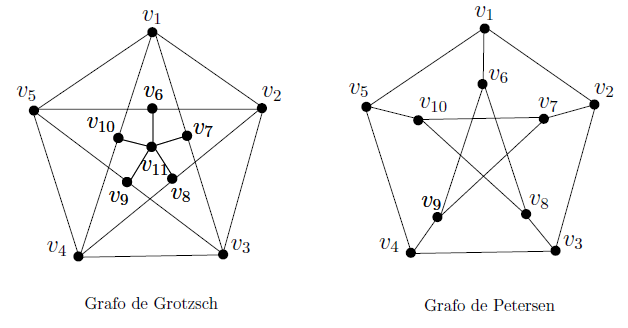
\includegraphics[scale=0.8]{Rel1}
%\end{figure}
%%
%%\newpage
%%
%%\begin{ejercicio}{1.12}
%%
%%\end{ejercicio}
%%\begin{solucion}
%%
%%\end{solucion}

\end{document}
